\chapter{Garment Pick and Place Points}
\label{pick_and_place}
This chapter explains the last stage of our algorithm, in which the pick and place points required for unfolding the current fold are determined. These points will be later sent to the humanoid robot to perform the unfolding operation. This stage has as input the clustered depth map obtained in the clustering stage (described in chapter \ref{garment_clustering}), and the garment approximated polygon (calculated in section \ref{segmentation_approximated_polygon}). Figure \ref{fig:garment_pnp_points_blocks} shows the block diagram of the different steps that are performed in this stage.

\begin{figure}[thpb]
    \centering
    
\includegraphics[width=0.7
    \textwidth]{figures/placeholder2.png}
    \caption{\comment{(Block diagram for Garment Depth Map Clustering chapter)}}
    \label{fig:garment_pnp_points_blocks}
\end{figure}

\section{Candidate Unfold Paths}
\label{unfold_paths}

Based in the assumption that when a garment has an overlapping fold, the fold line will rest in the garment contour, and the folded surface will have lower depth values (i.e. closer to the depth sensor), the next step in our algorithm is to create a set of paths from the highest point in the garment to the midpoint of each contour segment. These paths will be later analyzed using the clusters previously found in the depth image to select the path with less height variation.

To find the highest point in the garment, the clusters previously found with the Watershed algorithm are averaged using the median value for each cluster. Then, the region with the lowest depth value, which is closer to the camera and therefore higher in the garment, is selected as overlapping fold based on the previous assumption. The centroid of the selected cluster is the point selected as highest point. Using this method instead of selecting directly the highest point from the depth image increases the robustness of the algorithm against outliers and noise present in the depth image.

The midpoint of each segment of the garment approximated polygon is then calculated, and a set of paths departing from the highest point and arriving to the midpoints is created.

These paths are checked so that they are located entirely inside the garment, paths that go outside the garment approximated polygon are considered invalid. Figure \ref{fig:candidate_paths} shows both the initial paths set and the unfold candidate paths set, without the invalid paths.

\begin{figure}[thpb]
    \centering
    
\includegraphics[width=0.7
    \textwidth]{figures/placeholder2.png}
    \caption{\comment{(Figure that shows both the initial path candidate set and the candidate set without the invalid paths)}}
    \label{fig:candidate_paths}
\end{figure}

\section{Bumpiness}
\label{bumpiness}
Each of the candidate paths calculated using the method explained in the previous section has to be analyzed in this step to determine the best unfolding path. 

Prior to this analysis, each of the candidate paths is discretized in constant-length segments, and the depth image is sampled at those discrete points. This results in several n-dimensional vectors of depth samples to be analyzed. As the different paths may differ in length, the amount of sampled points and, therefore, the length of each of the vectors (i.e. $n$) will be different for each path. Figure \ref{fig:paths_with_bumpiness} shows the sample vector corresponding to each candidate path for a certain garment example.

The differences in depth between the overlapping fold region and the rest of the clothing article are assumed to be greater than the diferences in depth within the fold region \comment{points}. Under that assumption, the metric to evaluate the best path is a \textit{bumpiness} value \textit{B}, which is calculated by penalizing the changes in depth along each of the candidate sample vectors, as shown in Equation \ref{eq:bumpiness}.

\begin{equation}\label{eq:bumpiness}
B = \sum_{i=1}^{n} | \textrm{path}(i)- \textrm{path}(i-1) | 
\end{equation}

\comment{(Using path in the formula may confuse the reader, since we are using the sampled values and not the path itself)}

Where $n$ is the number of points composing the path. The path with the lowest bumpiness value, which corresponds to the path with the least and smallest height changes, is selected as the unfold direction, as shown in Figure \ref{fig:paths_with_bumpiness}.

\begin{figure}[thpb]
    \centering
    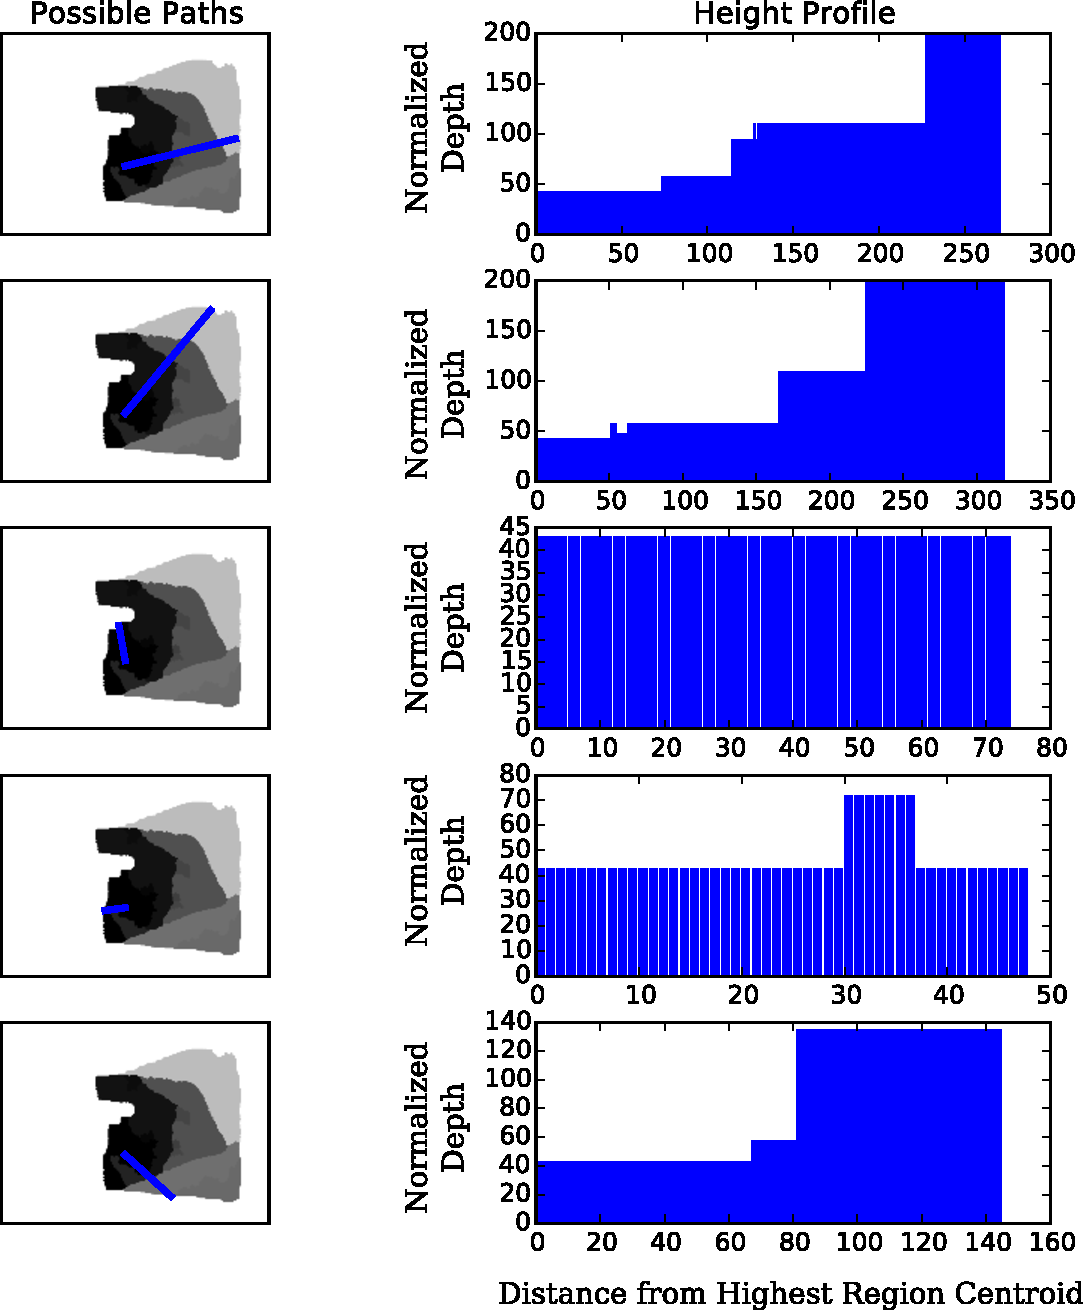
\includegraphics[width=\textwidth]{figures/candidate_paths.pdf}
    \caption{On the left side, the candidate paths are shown. On the right side, the height profile of each path is shown. Notice that the depth sensor computes the distance to the object from itself, so that a low value in the bar plot means a closer object to the sensor, so it is a region with more height with respect to the table.}
    \label{fig:paths_with_bumpiness}
\end{figure}

\section{Pick and Place Points}
\label{pick_and_place}
Once the most promising path for unfolding has been identified, the last step is to obtain pick and place points for the robot to perform the unfold action.

The most suitable grasping point for the picking action is located in the  intersection between the unfolding path direction line and the highest garment region border. This point is obtained by calculating the intersection between the selected path line and the highest region contour, selecting the point which is furthest to the garment border.

The other point is used as axis for a point reflection. To find the placing point, a reflection transformation is applied to the picking point using the aforementioned point as axis. Figure \ref{fig:directions} shows the unfold directions for several clothes, departing at the picking points and arriving to the placing points.

\begin{figure}[thpb]
    \centering
    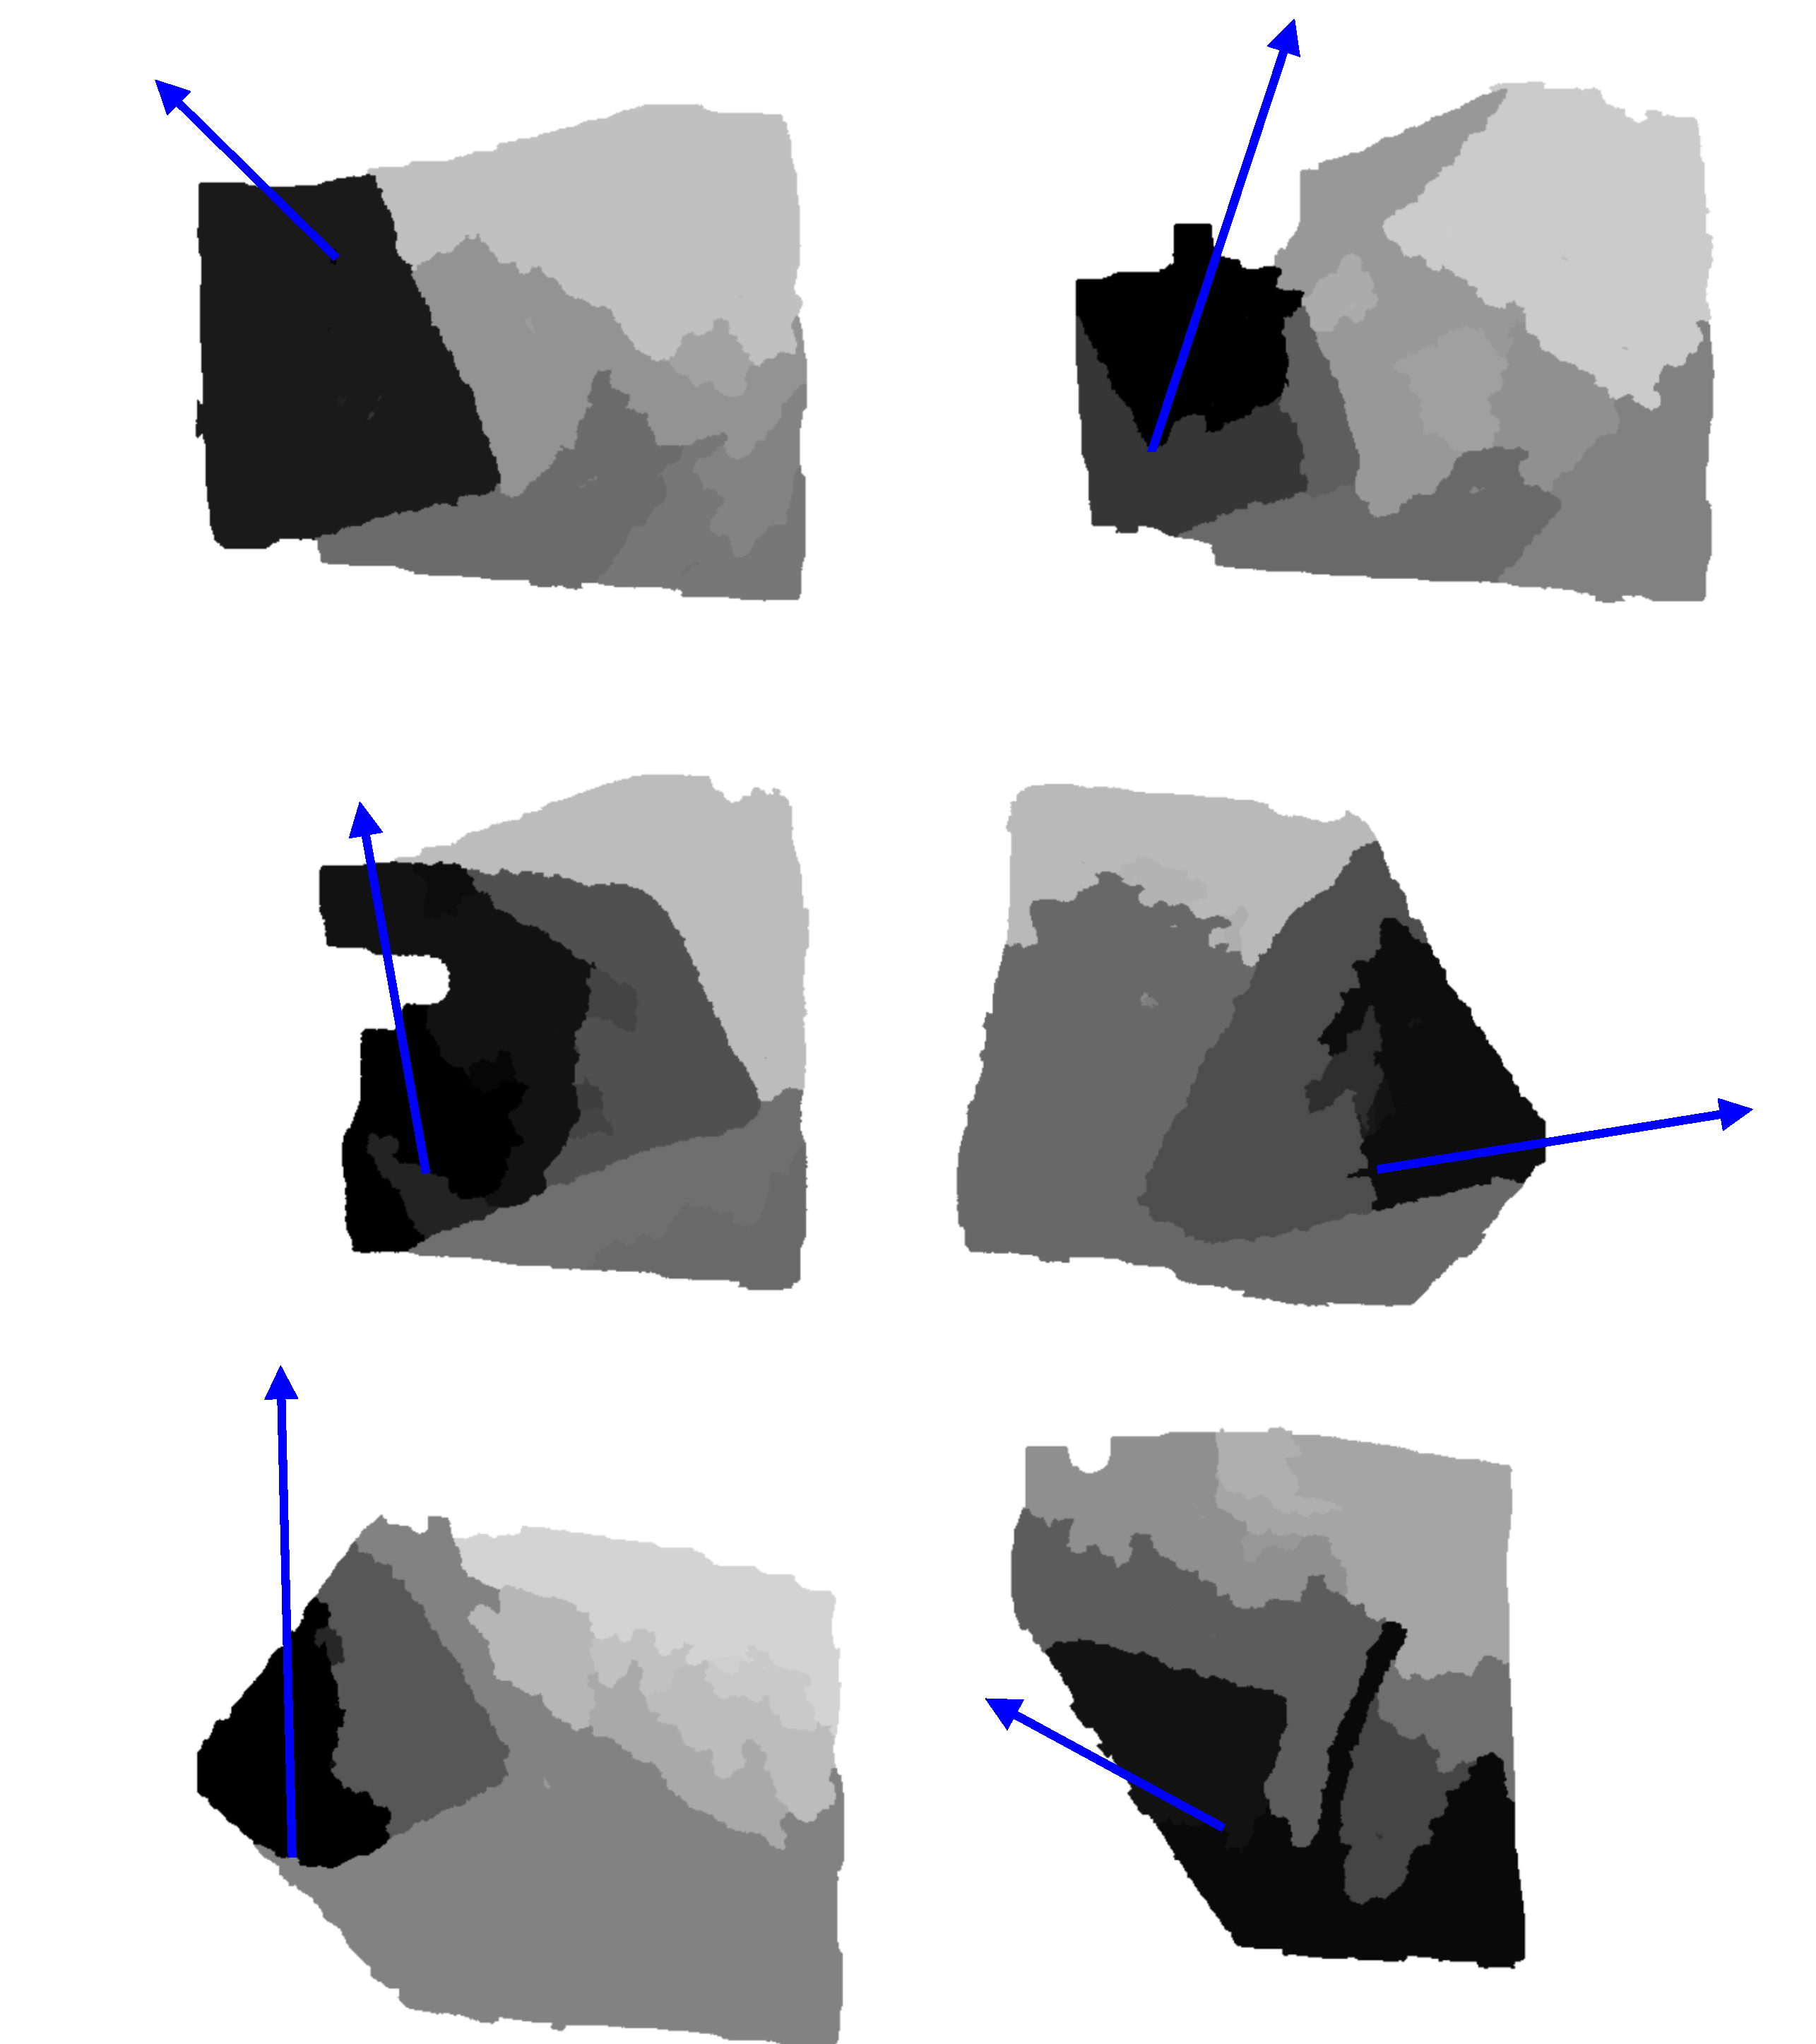
\includegraphics[width=0.7\textwidth]{figures/directions.pdf}
    \caption{Final directions calculated for each garment provided to the system. Each arrow departs where the robot should pick the fold and arrives where it should be placed.}
    \label{fig:directions}
\end{figure}

\warning{Moved from old \ref{garment_PnP_points} to here}

\comment{On the labeled watershed image, we calculate the average height value of each region, and assign this average value to all points in the region. The region with the highest average height is selected for further analysis. }

\comment{The next step, after having labeled the similar-height regions and found the highest region, is to find the unfold direction. The assumption made here is that the fold has at least one contour edge which is also a border of the garment. }

\comment{A set of candidate paths is generated, all of them starting at the centroid of the highest region, and ending in each contour segment midpoint. Each candidate path is analyzed and assigned a value calculated by penalizing the changes in the height of the path.}

\comment{Up to here, we have detected the most promising direction to unfold. Finally, we need to define is the exact point where the robot has to pick the garment, and the place point. }

\comment{For this, we extend the previously selected direction line. The garment pick point is chosen at the intersection of the direction line with the inner region border. To find this point, we compute the intersection between the line and the region contour, and select the point furthest to the garment border. }

\comment{On the other side, the place point is selected by computing the symmetric point of the pick point with respect to the garment edge intersection point. The unfold directions, departing from the pick point and arriving at the place point of a set of clothes, is shown in Fig. \ref{fig:directions}. }